\documentclass{article}
\usepackage[utf8]{inputenc}
\usepackage[spanish]{babel}
\usepackage{amsmath}
\usepackage{amssymb}
\usepackage{enumitem}
\usepackage{graphicx}

\title{Cortes, Ceros y Transformaciones}
\author{}
\date{}

\begin{document}

\maketitle

\section*{Ejercicio 1 (1.2.7)}

\textbf{Determine el tipo de singularidades (en caso de poseerlas) de las siguientes funciones en: $z = 0$ y $z = \infty$}

\subsection*{a) $f(z) = \frac{1}{z - 2}$}

Para analizar las singularidades, primero identificamos los puntos donde la función no está definida o no es analítica.

\subsubsection*{Análisis en $z = 0$:}

La función $f(z) = \frac{1}{z - 2}$ está definida en $z = 0$:
$$f(0) = \frac{1}{0 - 2} = \frac{1}{-2} = -\frac{1}{2}$$

Como $f(0)$ existe y es finito, y la función es analítica en una vecindad de $z = 0$ (excepto en $z = 2$), entonces $z = 0$ \textbf{NO es una singularidad}.

\subsubsection*{Análisis en $z = 2$:}

La función tiene un punto donde no está definida: $z = 2$. En este punto:
$$\lim_{z \to 2} f(z) = \lim_{z \to 2} \frac{1}{z - 2} = \infty$$

Por lo tanto, $z = 2$ es una \textbf{singularidad aislada}. 

La función puede escribirse como $f(z) = \frac{1}{z - 2}$, donde el denominador tiene un cero simple en $z = 2$. Por lo tanto, $z = 2$ es un \textbf{polo simple} (polo de orden 1).

\subsubsection*{Análisis en $z = \infty$:}

Evaluando el límite cuando $z \to \infty$:
$$\lim_{z \to \infty} f(z) = \lim_{z \to \infty} \frac{1}{z - 2} = \frac{1}{\infty} = 0$$

Como el límite existe y es finito (igual a 0), entonces $z = \infty$ es un \textbf{punto regular} (no es una singularidad).

\textbf{Resumen:}
\begin{itemize}
\item $z = 0$: \textbf{No es singularidad} (punto regular)
\item $z = 2$: \textbf{Polo simple} (singularidad aislada de orden 1)
\item $z = \infty$: \textbf{No es singularidad} (punto regular)
\end{itemize}

\subsection*{b) $f(z) = \frac{1 + z^3}{z^2}$}

\subsubsection*{Análisis en $z = 0$:}

La función $f(z) = \frac{1 + z^3}{z^2}$ no está definida en $z = 0$ porque el denominador se anula.

Evaluando el numerador en $z = 0$:
$$1 + z^3\Big|_{z=0} = 1 + 0 = 1 \neq 0$$

Como el numerador no se anula en $z = 0$ y el denominador tiene un cero de orden 2, entonces $z = 0$ es un \textbf{polo de orden 2}.

Verificando el límite:
$$\lim_{z \to 0} f(z) = \lim_{z \to 0} \frac{1 + z^3}{z^2} = \infty$$

\subsubsection*{Análisis en $z = \infty$:}

Evaluando el límite cuando $z \to \infty$:
$$\lim_{z \to \infty} f(z) = \lim_{z \to \infty} \frac{1 + z^3}{z^2} = \lim_{z \to \infty} \frac{z^3}{z^2} = \lim_{z \to \infty} z = \infty$$

Como el límite es infinito, $z = \infty$ es una \textbf{singularidad}. Dado que el grado del numerador (3) es mayor que el grado del denominador (2), $z = \infty$ es un \textbf{polo} (de orden 1, ya que el grado del numerador menos el del denominador es 1).

\textbf{Resumen:}
\begin{itemize}
\item $z = 0$: \textbf{Polo de orden 2}
\item $z = \infty$: \textbf{Polo} (singularidad)
\end{itemize}

\subsection*{c) $f(z) = \sinh\left(\frac{1}{z}\right)$}

\subsubsection*{Análisis en $z = 0$:}

La función $f(z) = \sinh\left(\frac{1}{z}\right)$ no está definida en $z = 0$ porque $\frac{1}{z}$ no está definido en $z = 0$.

Cuando $z \to 0$, tenemos que $\frac{1}{z} \to \infty$. La función $\sinh(w)$ tiene un comportamiento oscilatorio cuando $w \to \infty$ (o $w \to -\infty$), ya que:
$$\sinh(w) = \frac{e^w - e^{-w}}{2}$$

Cuando $w = \frac{1}{z} \to \infty$, el término $e^w$ domina y crece exponencialmente, mientras que cuando $w \to -\infty$, el término $-e^{-w}$ domina. Esto implica que el límite $\lim_{z \to 0} \sinh\left(\frac{1}{z}\right)$ no existe (ni finito ni infinito).

Por lo tanto, $z = 0$ es una \textbf{singularidad esencial}.

\subsubsection*{Análisis en $z = \infty$:}

Evaluando el límite cuando $z \to \infty$:
$$\lim_{z \to \infty} f(z) = \lim_{z \to \infty} \sinh\left(\frac{1}{z}\right) = \sinh(0) = 0$$

Como el límite existe y es finito (igual a 0), entonces $z = \infty$ es un \textbf{punto regular} (no es una singularidad).

\textbf{Resumen:}
\begin{itemize}
\item $z = 0$: \textbf{Singularidad esencial}
\item $z = \infty$: \textbf{No es singularidad} (punto regular)
\end{itemize}

\newpage
\section*{Ejercicio 2 (1.2.7)}

\textbf{Identifique los ceros, polos y las singularidades esenciales de las siguientes funciones:}

\subsection*{a) $f(z) = \frac{z - 2}{z^2} \sin\left(\frac{1}{1 - z}\right)$}

Para analizar esta función, debemos identificar:
\begin{itemize}
\item \textbf{Ceros}: puntos donde $f(z) = 0$
\item \textbf{Polos}: singularidades donde $\lim_{z \to z_0} f(z) = \infty$
\item \textbf{Singularidades esenciales}: singularidades que no son polos ni removibles
\end{itemize}

\subsubsection*{Identificación de puntos problemáticos:}

La función $f(z) = \frac{z - 2}{z^2} \sin\left(\frac{1}{1 - z}\right)$ tiene los siguientes puntos donde puede haber problemas:
\begin{itemize}
\item $z = 0$: el denominador $z^2$ se anula
\item $z = 1$: el argumento del seno $\frac{1}{1 - z}$ no está definido
\item Puntos donde $\sin\left(\frac{1}{1 - z}\right) = 0$: estos serían ceros adicionales
\end{itemize}

\subsubsection*{Análisis de ceros:}

Un cero de $f(z)$ ocurre cuando $f(z) = 0$. Esto sucede cuando:
\begin{enumerate}
\item El numerador $z - 2 = 0$, es decir, $z = 2$
\item O cuando $\sin\left(\frac{1}{1 - z}\right) = 0$
\end{enumerate}

\textbf{Caso 1:} $z = 2$

Evaluando en $z = 2$:
$$f(2) = \frac{2 - 2}{2^2} \sin\left(\frac{1}{1 - 2}\right) = \frac{0}{4} \sin(-1) = 0$$

Sin embargo, debemos verificar si $z = 2$ es un cero simple o de orden mayor. Para esto, calculamos la derivada:
$$f'(z) = \frac{d}{dz}\left[\frac{z - 2}{z^2} \sin\left(\frac{1}{1 - z}\right)\right]$$

Usando la regla del producto:
$$f'(z) = \frac{d}{dz}\left(\frac{z - 2}{z^2}\right) \sin\left(\frac{1}{1 - z}\right) + \frac{z - 2}{z^2} \frac{d}{dz}\left[\sin\left(\frac{1}{1 - z}\right)\right]$$

Calculando:
$$\frac{d}{dz}\left(\frac{z - 2}{z^2}\right) = \frac{z^2 - 2z(z - 2)}{z^4} = \frac{z^2 - 2z^2 + 4z}{z^4} = \frac{-z^2 + 4z}{z^4} = \frac{4 - z}{z^3}$$

Y:
$$\frac{d}{dz}\left[\sin\left(\frac{1}{1 - z}\right)\right] = \cos\left(\frac{1}{1 - z}\right) \cdot \frac{1}{(1 - z)^2}$$

Evaluando $f'(2)$:
$$f'(2) = \frac{4 - 2}{2^3} \sin(-1) + \frac{0}{4} \cdot \cos(-1) \cdot \frac{1}{(-1)^2} = \frac{2}{8} \sin(-1) = \frac{1}{4}\sin(-1) \neq 0$$

Por lo tanto, $z = 2$ es un \textbf{cero simple} (de orden 1).

\textbf{Caso 2:} $\sin\left(\frac{1}{1 - z}\right) = 0$

El seno se anula cuando su argumento es un múltiplo entero de $\pi$:
$$\frac{1}{1 - z} = n\pi, \quad n \in \mathbb{Z}, \quad n \neq 0$$

Resolviendo para $z$:
$$1 - z = \frac{1}{n\pi}$$
$$z = 1 - \frac{1}{n\pi}, \quad n \in \mathbb{Z}, \quad n \neq 0$$

Estos son ceros adicionales, siempre que el numerador $z - 2 \neq 0$ en esos puntos. Verificando:
$$1 - \frac{1}{n\pi} = 2 \quad \Rightarrow \quad \frac{1}{n\pi} = -1 \quad \Rightarrow \quad n = -\frac{1}{\pi}$$

Como $-\frac{1}{\pi}$ no es un entero, no hay conflicto. Por lo tanto, los puntos $z = 1 - \frac{1}{n\pi}$ (con $n \in \mathbb{Z}$, $n \neq 0$) son también \textbf{ceros simples} de la función.

\subsubsection*{Análisis de polos:}

\textbf{Polo en $z = 0$:}

La función tiene un factor $\frac{1}{z^2}$ que sugiere un polo en $z = 0$. Sin embargo, debemos verificar el comportamiento de $\sin\left(\frac{1}{1 - z}\right)$ en $z = 0$:

En $z = 0$:
$$\sin\left(\frac{1}{1 - 0}\right) = \sin(1) \neq 0$$

Por lo tanto:
$$f(z) = \frac{z - 2}{z^2} \sin(1) = \frac{-2}{z^2} \sin(1) + \frac{1}{z} \sin(1)$$

Como el término dominante es $\frac{-2\sin(1)}{z^2}$, y $\sin(1) \neq 0$, entonces $z = 0$ es un \textbf{polo de orden 2}.

\subsubsection*{Análisis de singularidades esenciales:}

\textbf{Singularidad en $z = 1$:}

En $z = 1$, el argumento del seno $\frac{1}{1 - z}$ no está definido porque $1 - z = 0$.

Cuando $z \to 1$, tenemos $\frac{1}{1 - z} \to \infty$. La función $\sin(w)$ cuando $w \to \infty$ oscila entre $-1$ y $1$, por lo que no tiene límite (ni finito ni infinito).

Sin embargo, debemos considerar el factor completo. Cerca de $z = 1$:
$$f(z) = \frac{z - 2}{z^2} \sin\left(\frac{1}{1 - z}\right)$$

Cuando $z \to 1$:
$$\frac{z - 2}{z^2} \to \frac{1 - 2}{1^2} = -1$$

Y $\sin\left(\frac{1}{1 - z}\right)$ oscila cuando $z \to 1$. Por lo tanto, el límite $\lim_{z \to 1} f(z)$ no existe (ni finito ni infinito), lo que indica que $z = 1$ es una \textbf{singularidad esencial}.

\textbf{Resumen:}
\begin{itemize}
\item \textbf{Ceros:}
  \begin{itemize}
  \item $z = 2$: cero simple
  \item $z = 1 - \frac{1}{n\pi}$ para $n \in \mathbb{Z}$, $n \neq 0$: ceros simples
  \end{itemize}
\item \textbf{Polos:}
  \begin{itemize}
  \item $z = 0$: polo de orden 2
  \end{itemize}
\item \textbf{Singularidades esenciales:}
  \begin{itemize}
  \item $z = 1$: singularidad esencial
  \end{itemize}
\end{itemize}

\subsection*{b) $f(z) = e^{1/z}$}

\subsubsection*{Análisis de ceros:}

Para que $f(z) = 0$, necesitaríamos $e^{1/z} = 0$. Sin embargo, la función exponencial nunca se anula: $e^w \neq 0$ para cualquier $w \in \mathbb{C}$.

Por lo tanto, $f(z)$ \textbf{no tiene ceros}.

\subsubsection*{Análisis de polos:}

Un polo requiere que $\lim_{z \to z_0} f(z) = \infty$. 

En $z = 0$:
$$\lim_{z \to 0} e^{1/z}$$

Cuando $z \to 0$ por el eje real positivo, tenemos $\frac{1}{z} \to +\infty$, entonces $e^{1/z} \to +\infty$.

Cuando $z \to 0$ por el eje real negativo, tenemos $\frac{1}{z} \to -\infty$, entonces $e^{1/z} \to 0$.

Como los límites por diferentes caminos dan resultados diferentes, el límite no existe de manera única. Sin embargo, el límite no es simplemente infinito en todas las direcciones, por lo que $z = 0$ \textbf{no es un polo}.

En cualquier otro punto $z_0 \neq 0$, la función $e^{1/z}$ es analítica, por lo que no hay polos.

Por lo tanto, $f(z)$ \textbf{no tiene polos}.

\subsubsection*{Análisis de singularidades esenciales:}

En $z = 0$, la función $f(z) = e^{1/z}$ no está definida.

Como vimos, cuando $z \to 0$ por diferentes caminos, la función toma diferentes valores:
\begin{itemize}
\item Si $z \to 0^+$ (por el eje real positivo): $e^{1/z} \to +\infty$
\item Si $z \to 0^-$ (por el eje real negativo): $e^{1/z} \to 0$
\item Si $z \to 0$ por el eje imaginario: $e^{1/(iy)} = e^{-i/y}$ oscila
\end{itemize}

El comportamiento oscilatorio y la falta de un límite único (ni finito ni infinito) caracterizan una singularidad esencial. Por lo tanto, $z = 0$ es una \textbf{singularidad esencial}.

\textbf{Resumen:}
\begin{itemize}
\item \textbf{Ceros:} Ninguno
\item \textbf{Polos:} Ninguno
\item \textbf{Singularidades esenciales:} $z = 0$
\end{itemize}

\subsection*{c) $f(z) = \tan\left(\frac{1}{z}\right)$}

Recordemos que $\tan(w) = \frac{\sin(w)}{\cos(w)}$.

\subsubsection*{Análisis de ceros:}

Un cero de $f(z)$ ocurre cuando $\tan\left(\frac{1}{z}\right) = 0$, es decir, cuando $\sin\left(\frac{1}{z}\right) = 0$.

El seno se anula cuando su argumento es un múltiplo entero de $\pi$:
$$\frac{1}{z} = n\pi, \quad n \in \mathbb{Z}, \quad n \neq 0$$

Resolviendo para $z$:
$$z = \frac{1}{n\pi}, \quad n \in \mathbb{Z}, \quad n \neq 0$$

Estos son los \textbf{ceros} de la función. Para determinar el orden, calculamos la derivada:
$$f'(z) = \frac{d}{dz}\left[\tan\left(\frac{1}{z}\right)\right] = \sec^2\left(\frac{1}{z}\right) \cdot \left(-\frac{1}{z^2}\right) = -\frac{\sec^2\left(\frac{1}{z}\right)}{z^2}$$

En $z = \frac{1}{n\pi}$:
$$f'\left(\frac{1}{n\pi}\right) = -\frac{\sec^2(n\pi)}{(1/(n\pi))^2} = -\frac{1}{(1/(n\pi))^2} = -(n\pi)^2 \neq 0$$

Por lo tanto, cada $z = \frac{1}{n\pi}$ (con $n \in \mathbb{Z}$, $n \neq 0$) es un \textbf{cero simple}.

\subsubsection*{Análisis de polos:}

Un polo de $f(z)$ ocurre cuando $\cos\left(\frac{1}{z}\right) = 0$, ya que $\tan(w) = \frac{\sin(w)}{\cos(w)}$ y el denominador se anula.

El coseno se anula cuando su argumento es $\frac{\pi}{2} + k\pi$ para $k \in \mathbb{Z}$:
$$\frac{1}{z} = \frac{\pi}{2} + k\pi = \frac{\pi(2k + 1)}{2}, \quad k \in \mathbb{Z}$$

Resolviendo para $z$:
$$z = \frac{2}{\pi(2k + 1)}, \quad k \in \mathbb{Z}$$

En estos puntos, el numerador $\sin\left(\frac{1}{z}\right) = \sin\left(\frac{\pi(2k + 1)}{2}\right) = \pm 1 \neq 0$.

Por lo tanto, $z = \frac{2}{\pi(2k + 1)}$ (con $k \in \mathbb{Z}$) son \textbf{polos simples} de la función.

\subsubsection*{Análisis de singularidades esenciales:}

En $z = 0$, la función $f(z) = \tan\left(\frac{1}{z}\right)$ no está definida porque $\frac{1}{z}$ no está definido.

Cuando $z \to 0$, tenemos $\frac{1}{z} \to \infty$. La función $\tan(w)$ cuando $w \to \infty$ oscila entre $-\infty$ y $+\infty$ de manera no acotada, ya que:
$$\tan(w) = \frac{\sin(w)}{\cos(w)}$$

Cuando $w \to \infty$, tanto $\sin(w)$ como $\cos(w)$ oscilan, y su cociente puede tomar cualquier valor real. El límite $\lim_{z \to 0} \tan\left(\frac{1}{z}\right)$ no existe (ni finito ni infinito de manera única), lo que caracteriza una singularidad esencial.

Por lo tanto, $z = 0$ es una \textbf{singularidad esencial}.

\textbf{Resumen:}
\begin{itemize}
\item \textbf{Ceros:} $z = \frac{1}{n\pi}$ para $n \in \mathbb{Z}$, $n \neq 0$ (ceros simples)
\item \textbf{Polos:} $z = \frac{2}{\pi(2k + 1)}$ para $k \in \mathbb{Z}$ (polos simples)
\item \textbf{Singularidades esenciales:} $z = 0$
\end{itemize}

\newpage
\section*{Ejercicio 7}

\textbf{Demuestre que bajo la transformación $w = 1/z$, las imágenes de las rectas $y = x - 1$ y $y = 0$ son, respectivamente, el círculo $u^2 + v^2 - u - v = 0$ y la recta $v = 0$. Además:}
\begin{enumerate}
\item Dibuje las cuatro curvas
\item Determine las direcciones correspondientes a lo largo de estas curvas
\item Verifique la conformalidad del mapeo en el punto $z_0 = 1$
\end{enumerate}

\subsection*{Transformación $w = 1/z$}

Sea $z = x + iy$ y $w = u + iv$. La transformación es:
$$w = \frac{1}{z} = \frac{1}{x + iy} = \frac{x - iy}{x^2 + y^2} = \frac{x}{x^2 + y^2} - i\frac{y}{x^2 + y^2}$$

Por lo tanto:
\begin{align}
u &= \frac{x}{x^2 + y^2} \label{eq:u} \\
v &= -\frac{y}{x^2 + y^2} \label{eq:v}
\end{align}

También podemos expresar $x$ e $y$ en términos de $u$ y $v$:
$$w = u + iv = \frac{1}{z} = \frac{1}{x + iy}$$

Multiplicando ambos lados por $z$:
$$(u + iv)(x + iy) = 1$$
$$ux + iuy + ivx - vy = 1$$
$$(ux - vy) + i(uy + vx) = 1$$

Igualando partes real e imaginaria:
\begin{align}
ux - vy &= 1 \label{eq:real} \\
uy + vx &= 0 \label{eq:imag}
\end{align}

Resolviendo el sistema:
De (\ref{eq:imag}): $uy = -vx$, entonces $y = -\frac{vx}{u}$ (si $u \neq 0$)

Sustituyendo en (\ref{eq:real}):
$$ux - v\left(-\frac{vx}{u}\right) = ux + \frac{v^2x}{u} = 1$$
$$x\left(u + \frac{v^2}{u}\right) = 1$$
$$x = \frac{u}{u^2 + v^2}$$

Y:
$$y = -\frac{vx}{u} = -\frac{v}{u} \cdot \frac{u}{u^2 + v^2} = -\frac{v}{u^2 + v^2}$$

\subsection*{Transformación de la recta $y = x - 1$}

La recta en el plano $z$ es: $y = x - 1$, o equivalentemente $x - y = 1$.

Sustituyendo las expresiones de $x$ e $y$ en términos de $u$ y $v$:
$$x - y = \frac{u}{u^2 + v^2} - \left(-\frac{v}{u^2 + v^2}\right) = \frac{u + v}{u^2 + v^2} = 1$$

Multiplicando ambos lados por $u^2 + v^2$:
$$u + v = u^2 + v^2$$

Reordenando:
$$u^2 + v^2 - u - v = 0$$

Completando cuadrados:
$$u^2 - u + v^2 - v = 0$$
$$\left(u^2 - u + \frac{1}{4}\right) + \left(v^2 - v + \frac{1}{4}\right) = \frac{1}{2}$$
$$\left(u - \frac{1}{2}\right)^2 + \left(v - \frac{1}{2}\right)^2 = \left(\frac{1}{\sqrt{2}}\right)^2$$

Esta es la ecuación de un círculo con centro en $\left(\frac{1}{2}, \frac{1}{2}\right)$ y radio $\frac{1}{\sqrt{2}}$.

\textbf{Conclusión:} La recta $y = x - 1$ se transforma en el círculo $u^2 + v^2 - u - v = 0$ (o equivalentemente, el círculo con centro en $\left(\frac{1}{2}, \frac{1}{2}\right)$ y radio $\frac{1}{\sqrt{2}}$).

\subsection*{Transformación de la recta $y = 0$}

La recta en el plano $z$ es: $y = 0$ (el eje real).

Usando la ecuación (\ref{eq:v}):
$$v = -\frac{y}{x^2 + y^2}$$

Cuando $y = 0$:
$$v = -\frac{0}{x^2 + 0^2} = 0$$

Por lo tanto, $v = 0$ para todos los puntos de la recta $y = 0$ (excepto $z = 0$).

\textbf{Conclusión:} La recta $y = 0$ se transforma en la recta $v = 0$ (el eje real en el plano $w$).

\subsection*{Dibujo de las cuatro curvas}

\textbf{En el plano $z$:}
\begin{itemize}
\item \textbf{Recta 1:} $y = x - 1$: Es una recta con pendiente 1 que pasa por el punto $(0, -1)$ y $(1, 0)$.
\item \textbf{Recta 2:} $y = 0$: Es el eje real (eje $x$).
\end{itemize}

\textbf{En el plano $w$:}
\begin{itemize}
\item \textbf{Imagen de $y = x - 1$:} Círculo $u^2 + v^2 - u - v = 0$ con centro en $\left(\frac{1}{2}, \frac{1}{2}\right)$ y radio $\frac{1}{\sqrt{2}} \approx 0.707$.
\item \textbf{Imagen de $y = 0$:} Recta $v = 0$ (eje real en el plano $w$).
\end{itemize}

\begin{figure}[h]
\centering
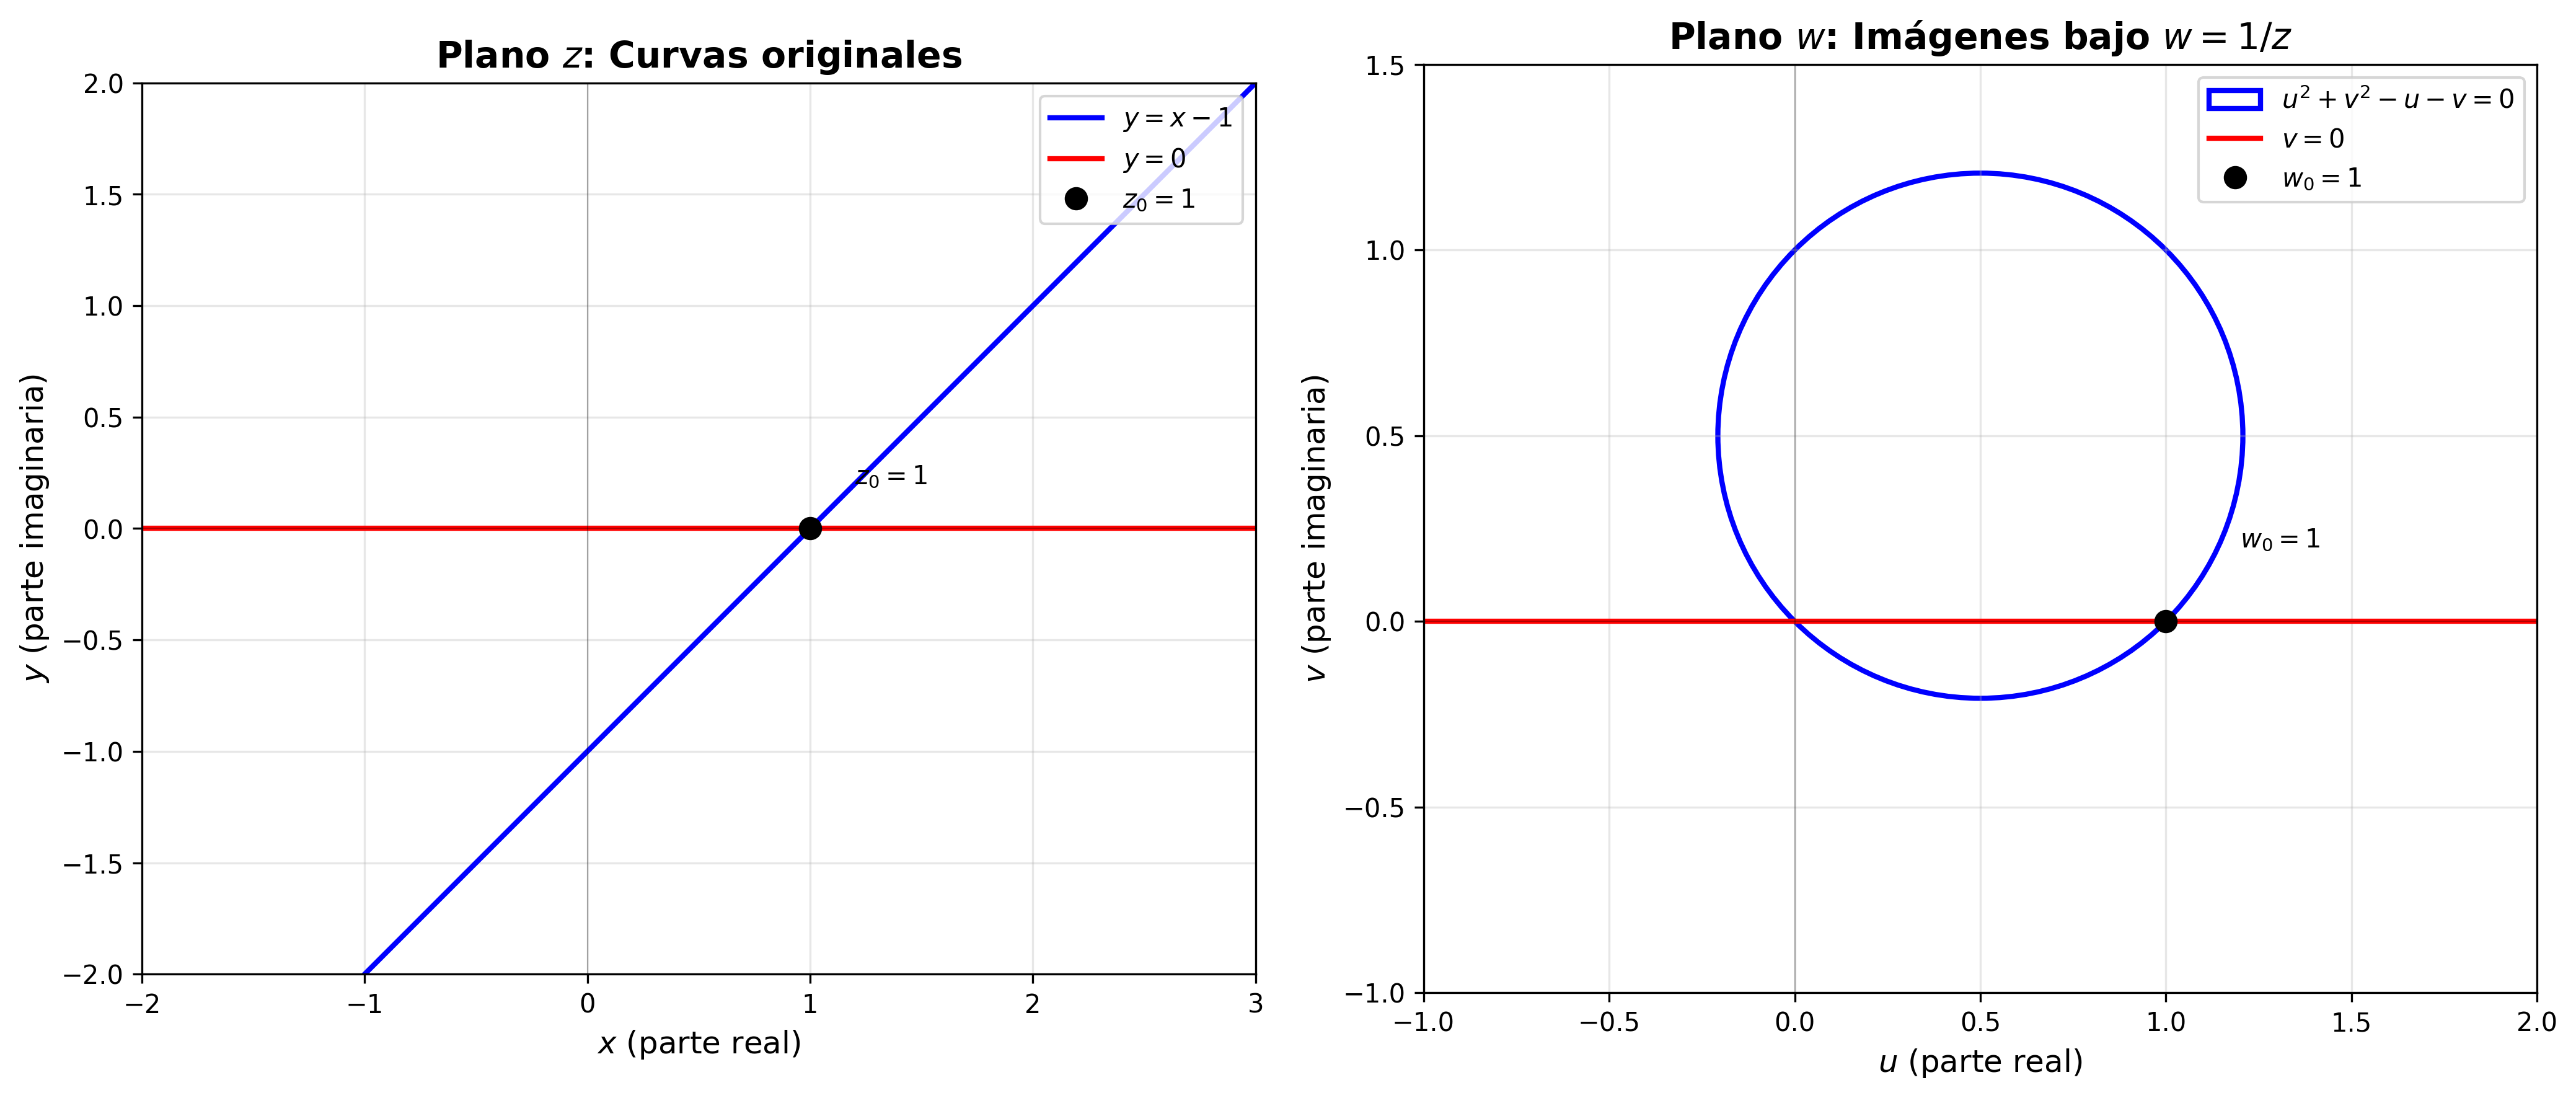
\includegraphics[width=0.9\textwidth]{../Codigos/transformacion_inversa_ejercicio7.png}
\caption{Curvas originales en el plano $z$ (izquierda) y sus imágenes transformadas en el plano $w$ bajo $w = 1/z$ (derecha).}
\label{fig:ejercicio7}
\end{figure}

\subsection*{Determinación de direcciones correspondientes}

Para determinar las direcciones, consideremos vectores tangentes a las curvas.

\textbf{En la recta $y = x - 1$:}

Un vector tangente es $\vec{t}_1 = (1, 1)$ (ya que la pendiente es 1).

\textbf{En la recta $y = 0$:}

Un vector tangente es $\vec{t}_2 = (1, 0)$ (a lo largo del eje $x$).

\textbf{Transformación de direcciones:}

La transformación $w = 1/z$ tiene derivada:
$$\frac{dw}{dz} = -\frac{1}{z^2}$$

Para un punto $z_0$ en la recta $y = x - 1$, la dirección se transforma según la derivada de la transformación. Sin embargo, es más útil considerar cómo se transforman los vectores tangentes.

Para un punto $z = x + i(x - 1)$ en la recta $y = x - 1$, tenemos:
$$w = \frac{1}{x + i(x - 1)} = \frac{x - i(x - 1)}{x^2 + (x - 1)^2} = \frac{x - i(x - 1)}{2x^2 - 2x + 1}$$

La dirección tangente en el plano $w$ se obtiene multiplicando el vector tangente por la derivada de la transformación.

\textbf{En la recta $y = 0$:}

Para un punto $z = x$ (real), tenemos $w = \frac{1}{x}$, que es también real. Por lo tanto, la dirección tangente $(1, 0)$ en el plano $z$ se mantiene como dirección tangente en el plano $w$ a lo largo del eje real $v = 0$.

\subsection*{Verificación de conformalidad en $z_0 = 1$}

Una transformación es conforme en un punto $z_0$ si preserva ángulos y la derivada $f'(z_0) \neq 0$.

Para $w = 1/z$, tenemos:
$$f'(z) = -\frac{1}{z^2}$$

En $z_0 = 1$:
$$f'(1) = -\frac{1}{1^2} = -1 \neq 0$$

Por lo tanto, la transformación es conforme en $z_0 = 1$.

\textbf{Verificación del ángulo:}

En $z_0 = 1$, las dos rectas se intersectan:
\begin{itemize}
\item Recta $y = x - 1$: en $z = 1$, tenemos $y = 1 - 1 = 0$, así que el punto es $(1, 0)$.
\item Recta $y = 0$: también pasa por $(1, 0)$.
\end{itemize}

El ángulo entre las rectas en $z = 1$:
\begin{itemize}
\item La recta $y = x - 1$ tiene dirección $(1, 1)$.
\item La recta $y = 0$ tiene dirección $(1, 0)$.
\end{itemize}

El ángulo $\theta$ entre estos vectores:
$$\cos(\theta) = \frac{(1, 1) \cdot (1, 0)}{|(1, 1)| \cdot |(1, 0)|} = \frac{1}{\sqrt{2} \cdot 1} = \frac{1}{\sqrt{2}}$$

Por lo tanto, $\theta = \frac{\pi}{4} = 45^\circ$.

\textbf{En el plano $w$:}

El punto $z = 1$ se transforma en:
$$w = \frac{1}{1} = 1$$

Es decir, el punto $(1, 0)$ en el plano $z$ se transforma en el punto $(1, 0)$ en el plano $w$.

En el plano $w$:
\begin{itemize}
\item La imagen del círculo $u^2 + v^2 - u - v = 0$ pasa por $w = 1$.
\item La recta $v = 0$ también pasa por $w = 1$.
\end{itemize}

Para verificar que el ángulo se preserva, calculamos las direcciones tangentes en $w = 1$:

Para el círculo $u^2 + v^2 - u - v = 0$, derivando implícitamente:
$$2u + 2v\frac{dv}{du} - 1 - \frac{dv}{du} = 0$$
$$(2v - 1)\frac{dv}{du} = 1 - 2u$$
$$\frac{dv}{du} = \frac{1 - 2u}{2v - 1}$$

En $w = 1$ (es decir, $u = 1, v = 0$):
$$\frac{dv}{du}\Big|_{(1,0)} = \frac{1 - 2(1)}{2(0) - 1} = \frac{-1}{-1} = 1$$

Por lo tanto, la dirección tangente al círculo en $w = 1$ es $(1, 1)$.

La recta $v = 0$ tiene dirección $(1, 0)$.

El ángulo entre $(1, 1)$ y $(1, 0)$ es:
$$\cos(\theta') = \frac{(1, 1) \cdot (1, 0)}{|(1, 1)| \cdot |(1, 0)|} = \frac{1}{\sqrt{2}}$$

Por lo tanto, $\theta' = \frac{\pi}{4} = 45^\circ$, que es el mismo ángulo que en el plano $z$.

\textbf{Conclusión:} La transformación preserva el ángulo en $z_0 = 1$, confirmando que es conforme en ese punto.

\newpage
\section*{Ejercicio 6}

\textbf{Determine el ángulo de rotación en el punto $z_0 = 2 + i$ cuando $w = z^2$, e ilústrelo para alguna curva particular. Demuestre que el factor de escala en ese punto es $2\sqrt{5}$.}

\subsection*{Ángulo de rotación}

Para la transformación $w = z^2$, la derivada es:
$$f'(z) = 2z$$

En el punto $z_0 = 2 + i$:
$$f'(2 + i) = 2(2 + i) = 4 + 2i$$

El ángulo de rotación está dado por el argumento de la derivada:
$$\text{Arg}(f'(z_0)) = \text{Arg}(4 + 2i) = \arctan\left(\frac{2}{4}\right) = \arctan\left(\frac{1}{2}\right)$$

Por lo tanto, el ángulo de rotación es $\arctan\left(\frac{1}{2}\right)$.

\subsection*{Ilustración con una curva particular}

Consideremos la curva $C$ en el plano $z$ que es una recta horizontal que pasa por $z_0 = 2 + i$, es decir, la recta $y = 1$.

Un vector tangente a esta curva en $z_0$ es $\vec{t} = (1, 0)$ (dirección horizontal).

Bajo la transformación $w = z^2$, este vector se transforma según la derivada. El vector tangente en el plano $w$ será:
$$\vec{t}_w = f'(z_0) \cdot \vec{t} = (4 + 2i) \cdot 1 = 4 + 2i$$

En coordenadas cartesianas, esto es $(4, 2)$.

El ángulo de rotación es la diferencia entre el argumento del vector transformado y el argumento del vector original:
$$\text{Arg}(4 + 2i) - \text{Arg}(1) = \arctan\left(\frac{2}{4}\right) - 0 = \arctan\left(\frac{1}{2}\right)$$

Esto confirma que el ángulo de rotación es $\arctan\left(\frac{1}{2}\right)$.

\subsection*{Factor de escala}

El factor de escala está dado por el módulo de la derivada:
$$|f'(z_0)| = |4 + 2i| = \sqrt{4^2 + 2^2} = \sqrt{16 + 4} = \sqrt{20} = 2\sqrt{5}$$

\textbf{Demostración alternativa:}

También podemos calcular directamente:
$$|f'(2 + i)| = |2(2 + i)| = 2|2 + i| = 2\sqrt{2^2 + 1^2} = 2\sqrt{4 + 1} = 2\sqrt{5}$$

Por lo tanto, el factor de escala en $z_0 = 2 + i$ es $2\sqrt{5}$.

\section*{Ejercicio 8}

\textbf{Demuestre que el ángulo de rotación en un punto distinto de cero $z_0 = r_0 e^{i\theta_0}$ bajo la transformación $w = z^n$ para $(n = 1, 2, \ldots)$, es $(n - 1)\theta_0$. Determine el factor de escala de la transformación en ese punto.}

\subsection*{Ángulo de rotación}

Para la transformación $w = z^n$, la derivada es:
$$f'(z) = nz^{n-1}$$

En el punto $z_0 = r_0 e^{i\theta_0}$:
$$f'(z_0) = n(r_0 e^{i\theta_0})^{n-1} = nr_0^{n-1} e^{i(n-1)\theta_0}$$

El ángulo de rotación está dado por el argumento de la derivada:
$$\text{Arg}(f'(z_0)) = \text{Arg}(nr_0^{n-1} e^{i(n-1)\theta_0}) = (n - 1)\theta_0$$

ya que $nr_0^{n-1} > 0$ (es un número real positivo).

\textbf{Demostración:} El argumento de $f'(z_0) = nr_0^{n-1} e^{i(n-1)\theta_0}$ es simplemente $(n - 1)\theta_0$ porque el factor $nr_0^{n-1}$ es real y positivo, por lo que no contribuye al argumento.

Por lo tanto, el ángulo de rotación es $(n - 1)\theta_0$.

\subsection*{Factor de escala}

El factor de escala está dado por el módulo de la derivada:
$$|f'(z_0)| = |nr_0^{n-1} e^{i(n-1)\theta_0}| = nr_0^{n-1}|e^{i(n-1)\theta_0}| = nr_0^{n-1}$$

ya que $|e^{i(n-1)\theta_0}| = 1$.

Por lo tanto, el factor de escala en $z_0 = r_0 e^{i\theta_0}$ es $nr_0^{n-1}$.

\textbf{Resumen:}
\begin{itemize}
\item \textbf{Ángulo de rotación:} $(n - 1)\theta_0$
\item \textbf{Factor de escala:} $nr_0^{n-1}$
\end{itemize}

\section*{Ejercicio 9}

\textbf{Demuestre que la transformación $w = \sin(z)$ es conforme en todos los puntos excepto en $z = \frac{\pi}{2} + n\pi$ ($n = 0, \pm 1, \pm 2, \ldots$).}

\subsection*{Condición de conformalidad}

Una transformación $w = f(z)$ es conforme en un punto $z_0$ si y solo si $f'(z_0) \neq 0$ y $f'(z_0)$ existe.

Para $w = \sin(z)$, la derivada es:
$$f'(z) = \cos(z)$$

\subsection*{Puntos donde la transformación es conforme}

La transformación es conforme en todos los puntos donde $f'(z) \neq 0$, es decir, donde:
$$\cos(z) \neq 0$$

Esto ocurre cuando:
$$z \neq \frac{\pi}{2} + n\pi, \quad n \in \mathbb{Z}$$

\subsection*{Puntos donde la transformación NO es conforme}

En los puntos $z = \frac{\pi}{2} + n\pi$ ($n = 0, \pm 1, \pm 2, \ldots$), tenemos:
$$f'\left(\frac{\pi}{2} + n\pi\right) = \cos\left(\frac{\pi}{2} + n\pi\right) = 0$$

Cuando la derivada es cero, la transformación no preserva ángulos (el factor de escala es cero), por lo que la transformación \textbf{NO es conforme} en estos puntos.

\subsection*{Verificación}

Para $n = 0$:
$$f'\left(\frac{\pi}{2}\right) = \cos\left(\frac{\pi}{2}\right) = 0$$

Para $n = 1$:
$$f'\left(\frac{\pi}{2} + \pi\right) = \cos\left(\frac{3\pi}{2}\right) = 0$$

Para $n = -1$:
$$f'\left(\frac{\pi}{2} - \pi\right) = \cos\left(-\frac{\pi}{2}\right) = 0$$

Y así sucesivamente para todos los enteros $n$.

\textbf{Conclusión:} La transformación $w = \sin(z)$ es conforme en todos los puntos del plano complejo excepto en $z = \frac{\pi}{2} + n\pi$ para $n = 0, \pm 1, \pm 2, \ldots$, donde la derivada se anula y la transformación no preserva ángulos.

\section*{Ejercicio 10}

\textbf{Encuentre la transformación inversa local de $w = z^2$ en los puntos (a) $z_0 = 2$; (b) $z_0 = -2$; (c) $z_0 = -i$.}

\subsection*{Transformación inversa local}

Para $w = z^2$, la transformación inversa es $z = \sqrt{w}$. Sin embargo, como la función $z^2$ no es inyectiva en todo el plano complejo, necesitamos considerar ramas locales de la función inversa.

La derivada de $f(z) = z^2$ es $f'(z) = 2z$. Para que exista una inversa local, necesitamos $f'(z_0) \neq 0$, es decir, $z_0 \neq 0$.

En los tres casos dados, $z_0 \neq 0$, por lo que existe una inversa local en cada punto.

\subsection*{(a) $z_0 = 2$}

En $z_0 = 2$:
$$w_0 = f(2) = 2^2 = 4$$

La derivada en este punto es:
$$f'(2) = 2(2) = 4 \neq 0$$

Por el teorema de la función inversa, existe una inversa local. La inversa local es:
$$z = \sqrt{w}$$

Para la rama que pasa por $z_0 = 2$, tomamos la rama principal del logaritmo. Como $z_0 = 2 > 0$ (real positivo), la inversa local es:
$$z = \sqrt{w} = w^{1/2}$$

donde usamos la rama que da $\sqrt{4} = 2$.

\textbf{Verificación:}
$$f^{-1}(4) = \sqrt{4} = 2 = z_0 \quad \checkmark$$

\subsection*{(b) $z_0 = -2$}

En $z_0 = -2$:
$$w_0 = f(-2) = (-2)^2 = 4$$

La derivada en este punto es:
$$f'(-2) = 2(-2) = -4 \neq 0$$

La inversa local es:
$$z = \sqrt{w}$$

Para la rama que pasa por $z_0 = -2$, necesitamos la rama que da $\sqrt{4} = -2$. Esto corresponde a la rama:
$$z = -\sqrt{w} = -w^{1/2}$$

donde $\sqrt{w}$ es la rama principal (que da valores positivos para $w$ real positivo).

\textbf{Verificación:}
$$f^{-1}(4) = -\sqrt{4} = -2 = z_0 \quad \checkmark$$

\subsection*{(c) $z_0 = -i$}

En $z_0 = -i$:
$$w_0 = f(-i) = (-i)^2 = i^2 = -1$$

La derivada en este punto es:
$$f'(-i) = 2(-i) = -2i \neq 0$$

La inversa local es:
$$z = \sqrt{w}$$

Para encontrar la rama correcta, expresamos $z_0 = -i$ en forma polar:
$$z_0 = -i = e^{-i\pi/2}$$

Y $w_0 = -1 = e^{i\pi}$.

Para la rama que pasa por $z_0 = -i$, necesitamos:
$$\sqrt{-1} = -i$$

Esto corresponde a:
$$z = \sqrt{w} = w^{1/2} = e^{\frac{1}{2}\text{Log}(w)}$$

donde $\text{Log}(w)$ es el logaritmo principal. Para $w = -1 = e^{i\pi}$:
$$\text{Log}(-1) = \ln|1| + i\pi = i\pi$$

Por lo tanto:
$$z = e^{\frac{1}{2}i\pi} = e^{i\pi/2} = i$$

Pero esto da $i$, no $-i$. Necesitamos usar una rama diferente. Si usamos:
$$z = e^{\frac{1}{2}(\text{Log}(w) + 2\pi i)} = e^{\frac{1}{2}(i\pi + 2\pi i)} = e^{\frac{3\pi i}{2}} = e^{-i\pi/2} = -i$$

O más simplemente, la inversa local es:
$$z = -\sqrt{w}$$

donde $\sqrt{w}$ es la rama principal. Para $w = -1$:
$$z = -\sqrt{-1} = -i = z_0 \quad \checkmark$$

\textbf{Resumen de las transformaciones inversas locales:}
\begin{itemize}
\item \textbf{(a) $z_0 = 2$:} $z = \sqrt{w}$ (rama principal)
\item \textbf{(b) $z_0 = -2$:} $z = -\sqrt{w}$ (rama negativa)
\item \textbf{(c) $z_0 = -i$:} $z = -\sqrt{w}$ (rama que da $-i$ para $w = -1$)
\end{itemize}

\newpage
\section*{Ejercicio 11}

\textbf{Dibuje o grafique la región dada y su imagen bajo las siguientes transformaciones:}

\subsection*{a) Región: $|z| \leq \frac{1}{2}$, $-\frac{\pi}{8} < \text{Arg}(z) < \frac{\pi}{8}$; Transformación: $w = z^2$}

\subsubsection*{Descripción de la región en el plano $z$:}

La región está definida por:
\begin{itemize}
\item $|z| \leq \frac{1}{2}$: disco cerrado de radio $\frac{1}{2}$ centrado en el origen
\item $-\frac{\pi}{8} < \text{Arg}(z) < \frac{\pi}{8}$: sector angular entre los ángulos $-\frac{\pi}{8}$ y $\frac{\pi}{8}$
\end{itemize}

Esta es una \textbf{cuña} (sector de disco) de radio máximo $\frac{1}{2}$ y ángulo de apertura $\frac{\pi}{4}$ (desde $-\frac{\pi}{8}$ hasta $\frac{\pi}{8}$).

\subsubsection*{Transformación bajo $w = z^2$:}

Si $z = re^{i\theta}$ con $r \leq \frac{1}{2}$ y $-\frac{\pi}{8} < \theta < \frac{\pi}{8}$, entonces:
$$w = z^2 = r^2 e^{i(2\theta)}$$

Por lo tanto:
\begin{itemize}
\item El módulo se transforma: $|w| = r^2 \leq \left(\frac{1}{2}\right)^2 = \frac{1}{4}$
\item El argumento se transforma: $\text{Arg}(w) = 2\theta$, entonces $-\frac{\pi}{4} < \text{Arg}(w) < \frac{\pi}{4}$
\end{itemize}

\textbf{Imagen en el plano $w$:} Una cuña de radio máximo $\frac{1}{4}$ y ángulo de apertura $\frac{\pi}{2}$ (desde $-\frac{\pi}{4}$ hasta $\frac{\pi}{4}$).

\begin{figure}[h]
\centering
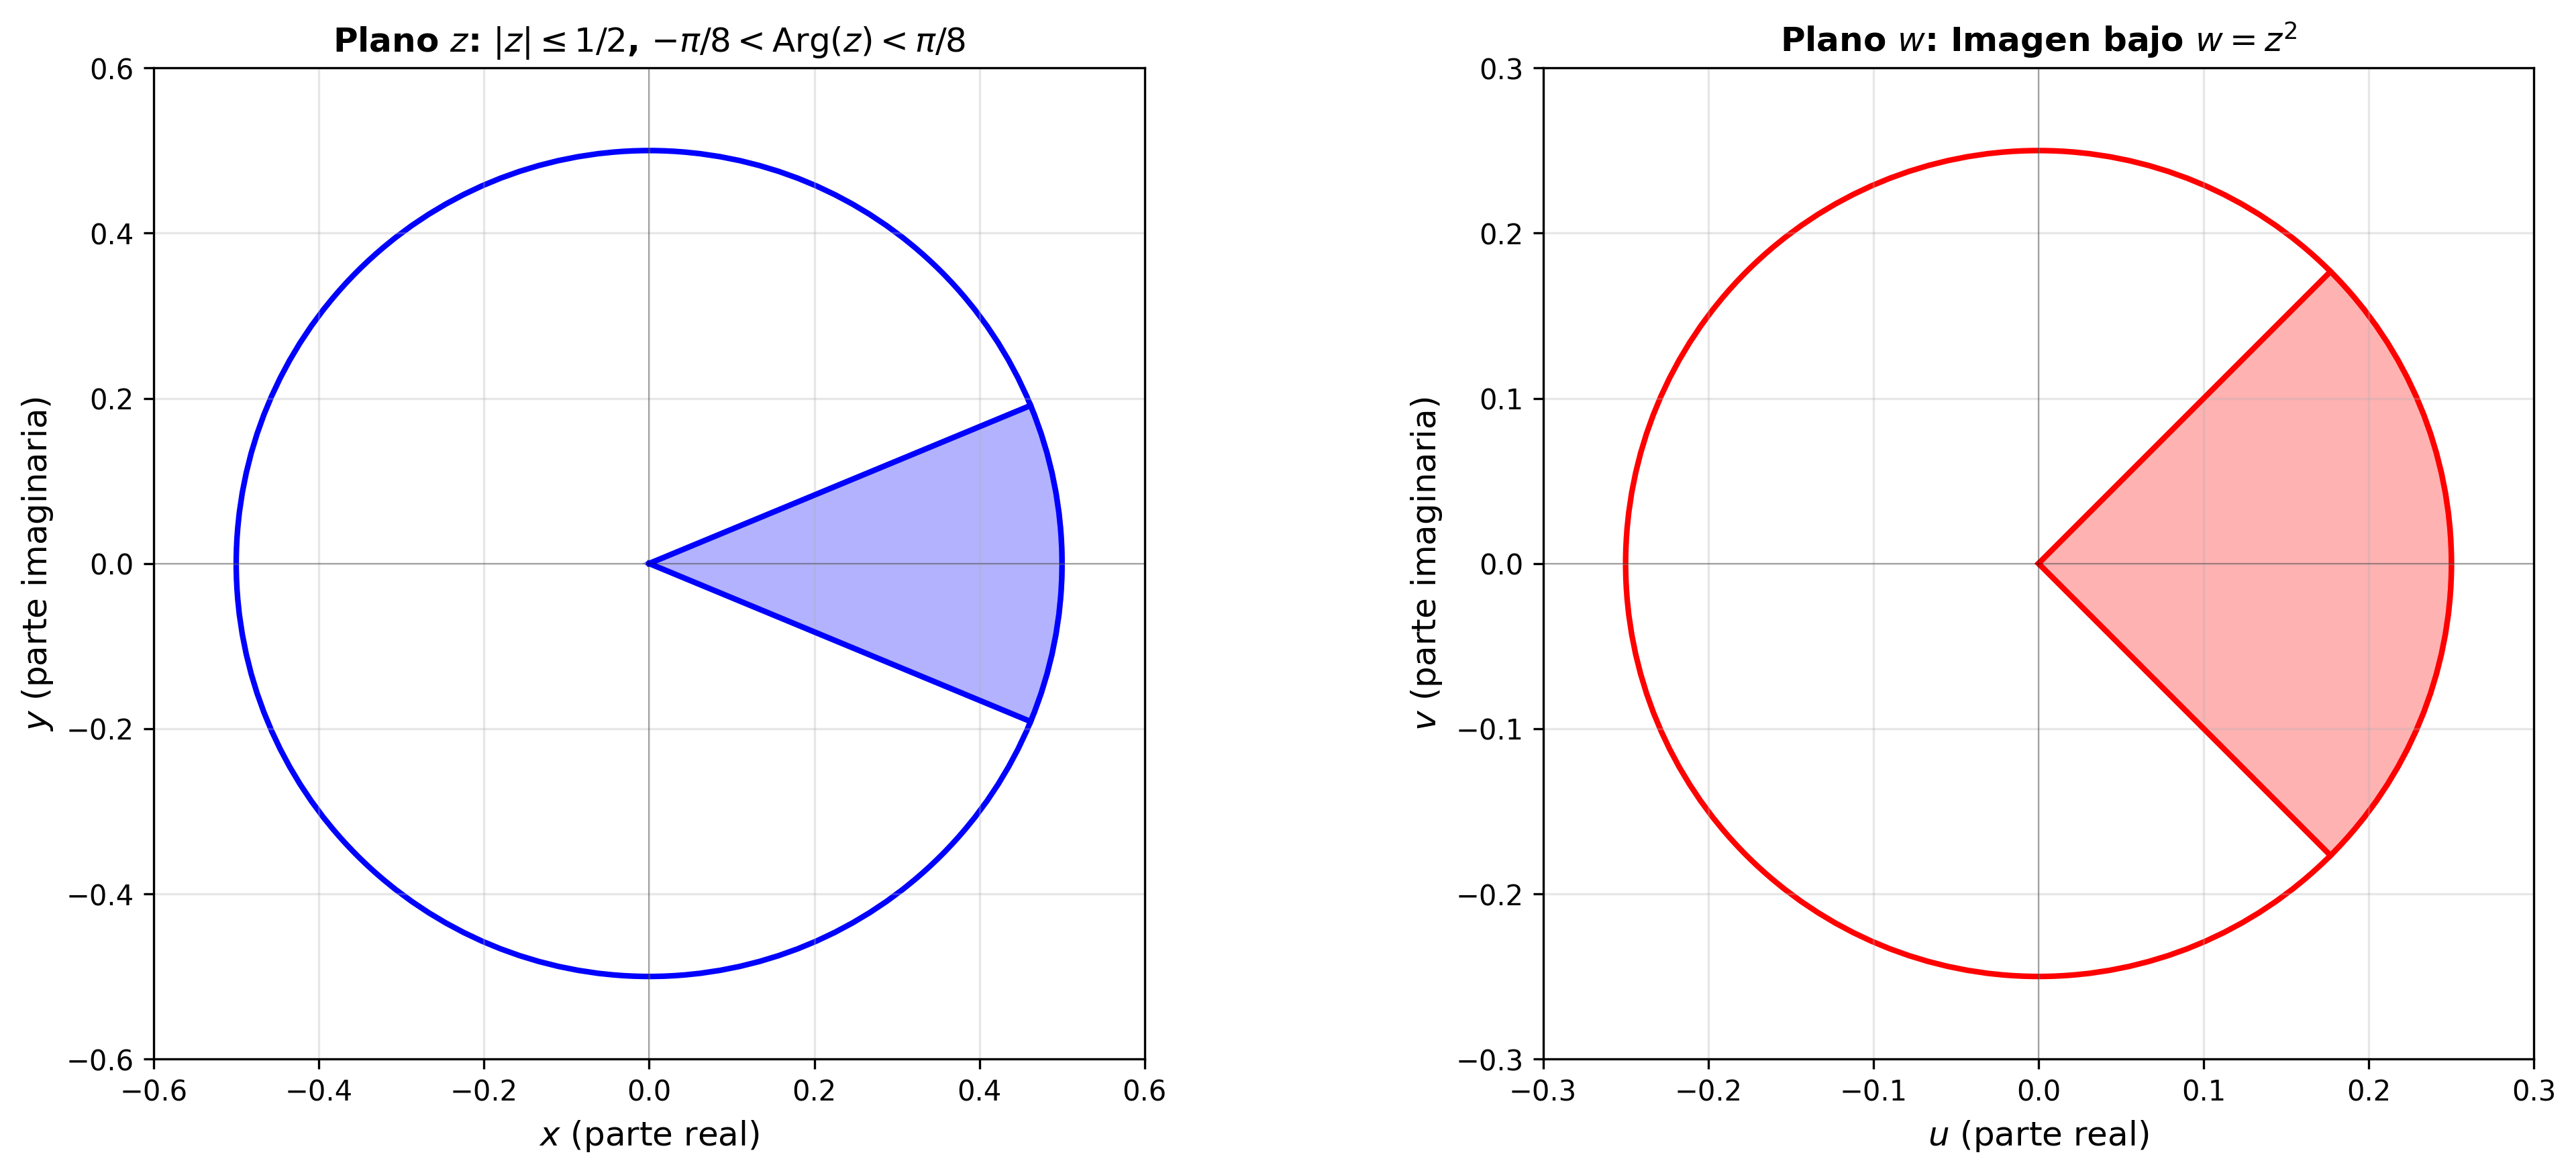
\includegraphics[width=0.9\textwidth]{../Codigos/ejercicio11a.png}
\caption{Región original (izquierda) e imagen transformada (derecha) para el ejercicio 11a.}
\label{fig:ejercicio11a}
\end{figure}

\subsection*{b) Región: $1 < |z| < 3$, $0 < \text{Arg}(z) < \frac{\pi}{2}$; Transformación: $w = z^3$}

\subsubsection*{Descripción de la región en el plano $z$:}

La región está definida por:
\begin{itemize}
\item $1 < |z| < 3$: anillo (corona circular) entre los círculos de radio 1 y 3 (sin incluir las fronteras)
\item $0 < \text{Arg}(z) < \frac{\pi}{2}$: primer cuadrante (sin incluir los ejes)
\end{itemize}

Esta es un \textbf{sector de anillo} en el primer cuadrante.

\subsubsection*{Transformación bajo $w = z^3$:}

Si $z = re^{i\theta}$ con $1 < r < 3$ y $0 < \theta < \frac{\pi}{2}$, entonces:
$$w = z^3 = r^3 e^{i(3\theta)}$$

Por lo tanto:
\begin{itemize}
\item El módulo se transforma: $1^3 < |w| < 3^3$, es decir, $1 < |w| < 27$
\item El argumento se transforma: $\text{Arg}(w) = 3\theta$, entonces $0 < \text{Arg}(w) < \frac{3\pi}{2}$
\end{itemize}

\textbf{Imagen en el plano $w$:} Un sector de anillo con radios entre 1 y 27, y ángulo que va desde $0$ hasta $\frac{3\pi}{2}$ (cubre el primer, segundo y parte del tercer cuadrante).

\begin{figure}[h]
\centering
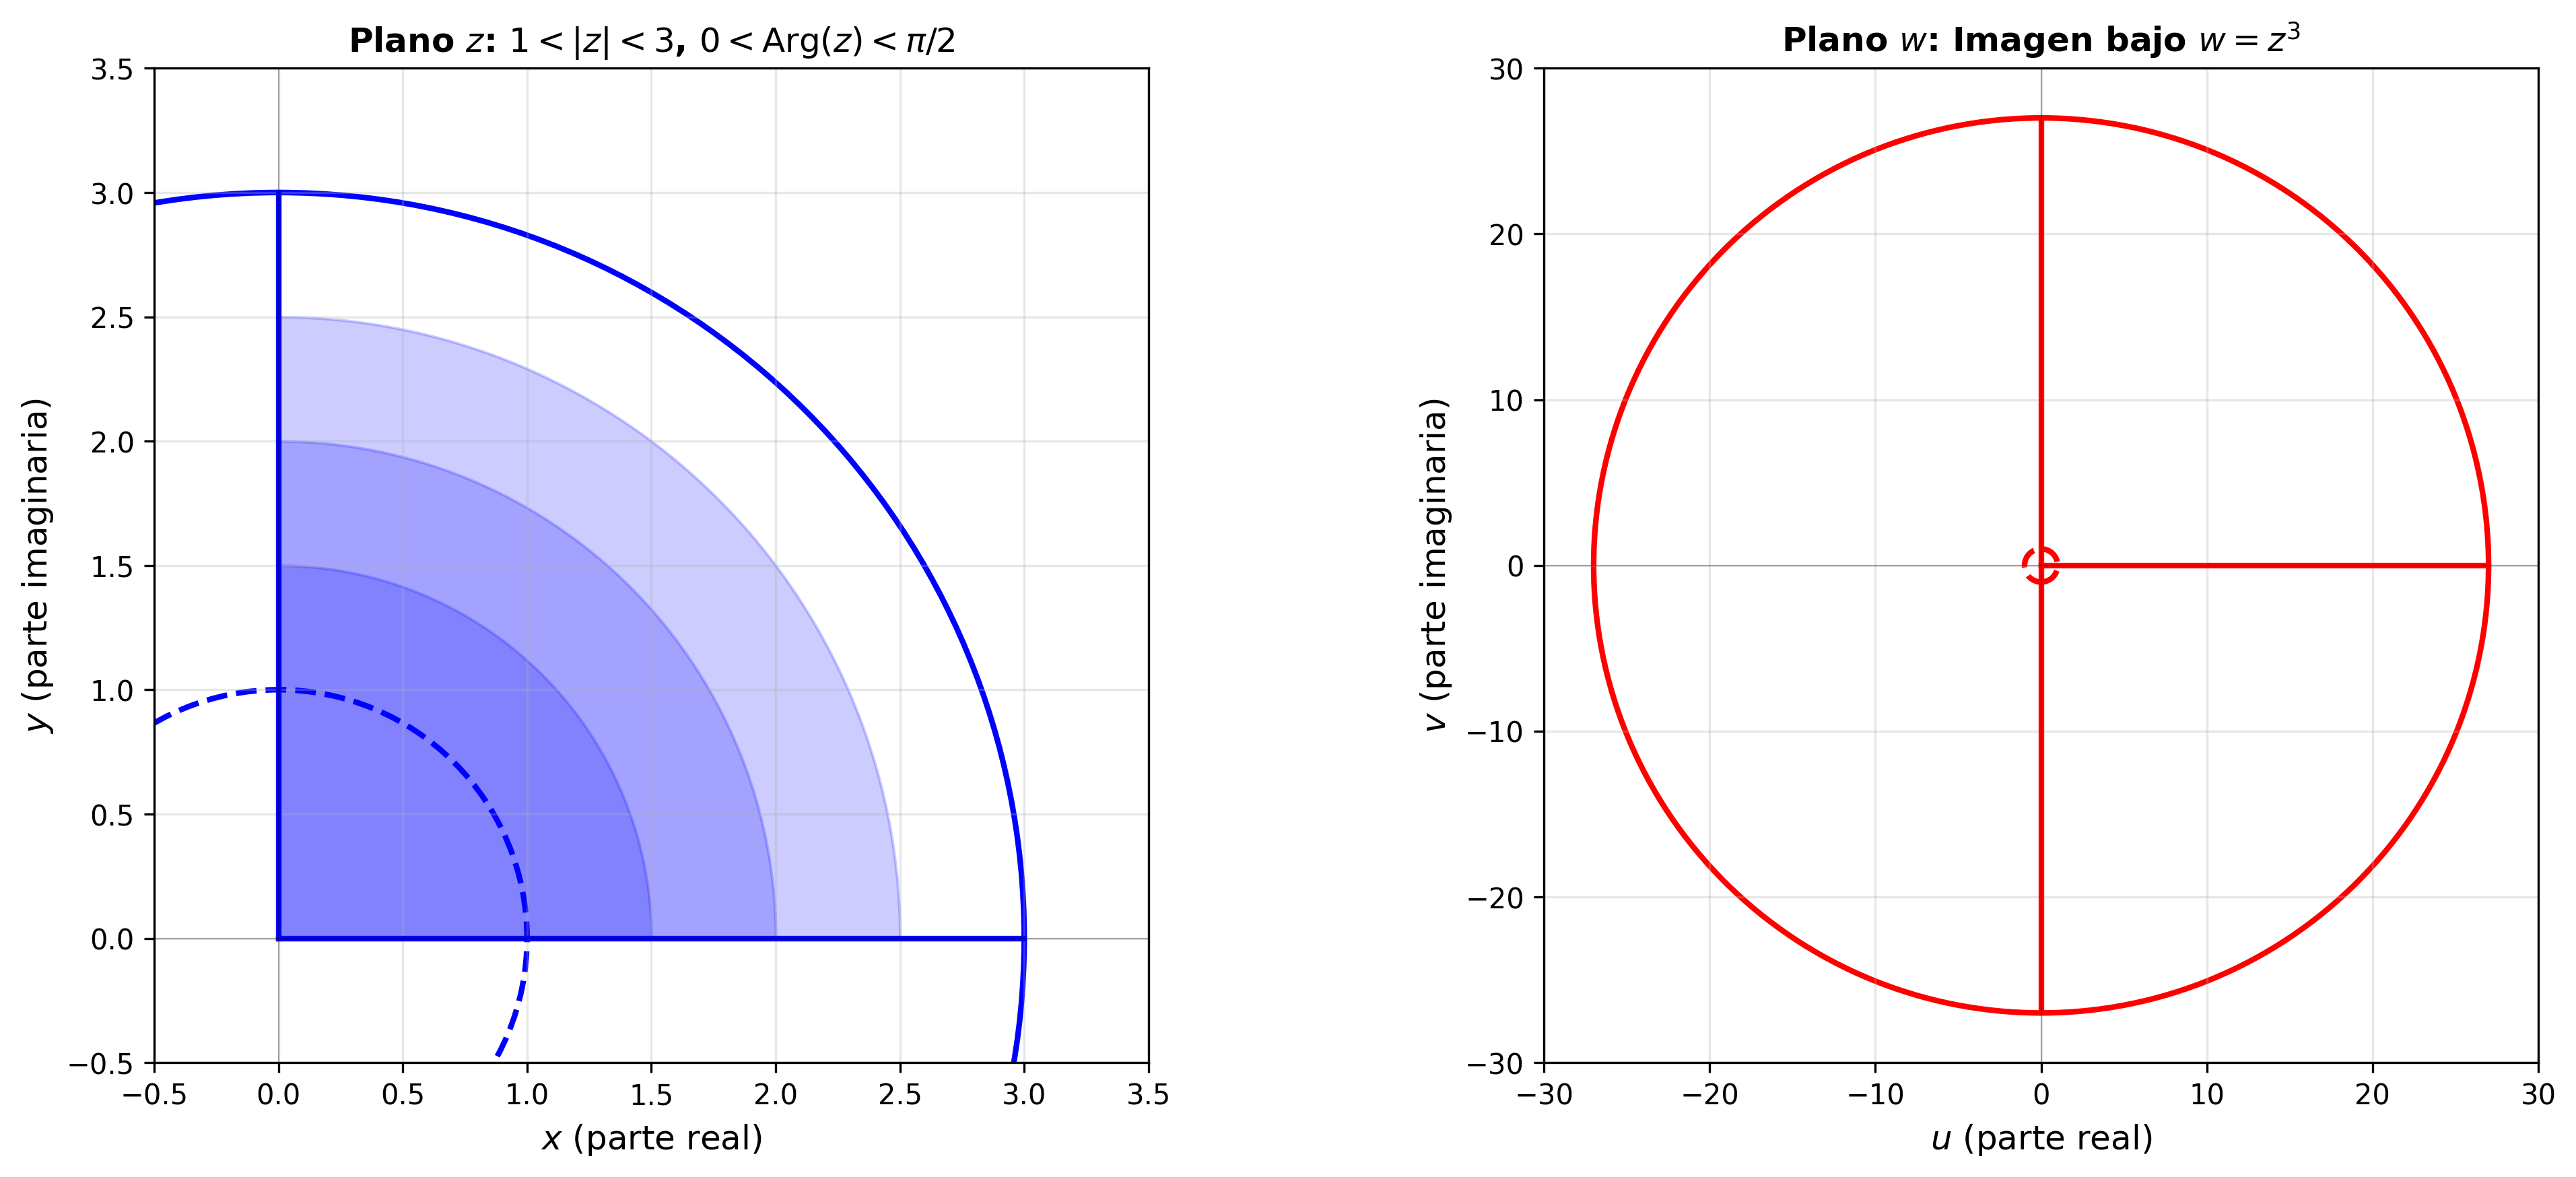
\includegraphics[width=0.9\textwidth]{../Codigos/ejercicio11b.png}
\caption{Región original (izquierda) e imagen transformada (derecha) para el ejercicio 11b.}
\label{fig:ejercicio11b}
\end{figure}

\subsection*{c) Región: $2 \leq \text{Im}(z) \leq 5$; Transformación: $w = z^3$}

\subsubsection*{Descripción de la región en el plano $z$:}

La región está definida por:
\begin{itemize}
\item $2 \leq \text{Im}(z) \leq 5$: banda horizontal entre las rectas $y = 2$ y $y = 5$ (incluyendo las fronteras)
\item No hay restricción en $\text{Re}(z)$, por lo que se extiende infinitamente en la dirección horizontal
\end{itemize}

Esta es una \textbf{banda horizontal} de ancho 3 unidades.

\subsubsection*{Transformación bajo $w = z^3$:}

Si $z = x + iy$ con $2 \leq y \leq 5$ y $x \in \mathbb{R}$, entonces:
$$w = z^3 = (x + iy)^3 = x^3 + 3ix^2y - 3xy^2 - iy^3 = (x^3 - 3xy^2) + i(3x^2y - y^3)$$

Por lo tanto:
\begin{align*}
u &= \text{Re}(w) = x^3 - 3xy^2 \\
v &= \text{Im}(w) = 3x^2y - y^3
\end{align*}

Para analizar la imagen, consideremos curvas paramétricas:
\begin{itemize}
\item Para $y = 2$ (frontera inferior): $u = x^3 - 12x$, $v = 12x^2 - 8$
\item Para $y = 5$ (frontera superior): $u = x^3 - 75x$, $v = 75x^2 - 125$
\end{itemize}

Cuando $x \to \pm \infty$, tanto $u$ como $v$ tienden a $\pm \infty$ dependiendo del signo de $x$.

\textbf{Imagen en el plano $w$:} Una región compleja que se extiende infinitamente. Las fronteras $y = 2$ y $y = 5$ se transforman en curvas cúbicas en el plano $w$. La región completa es el área entre estas dos curvas cúbicas.

\begin{figure}[h]
\centering
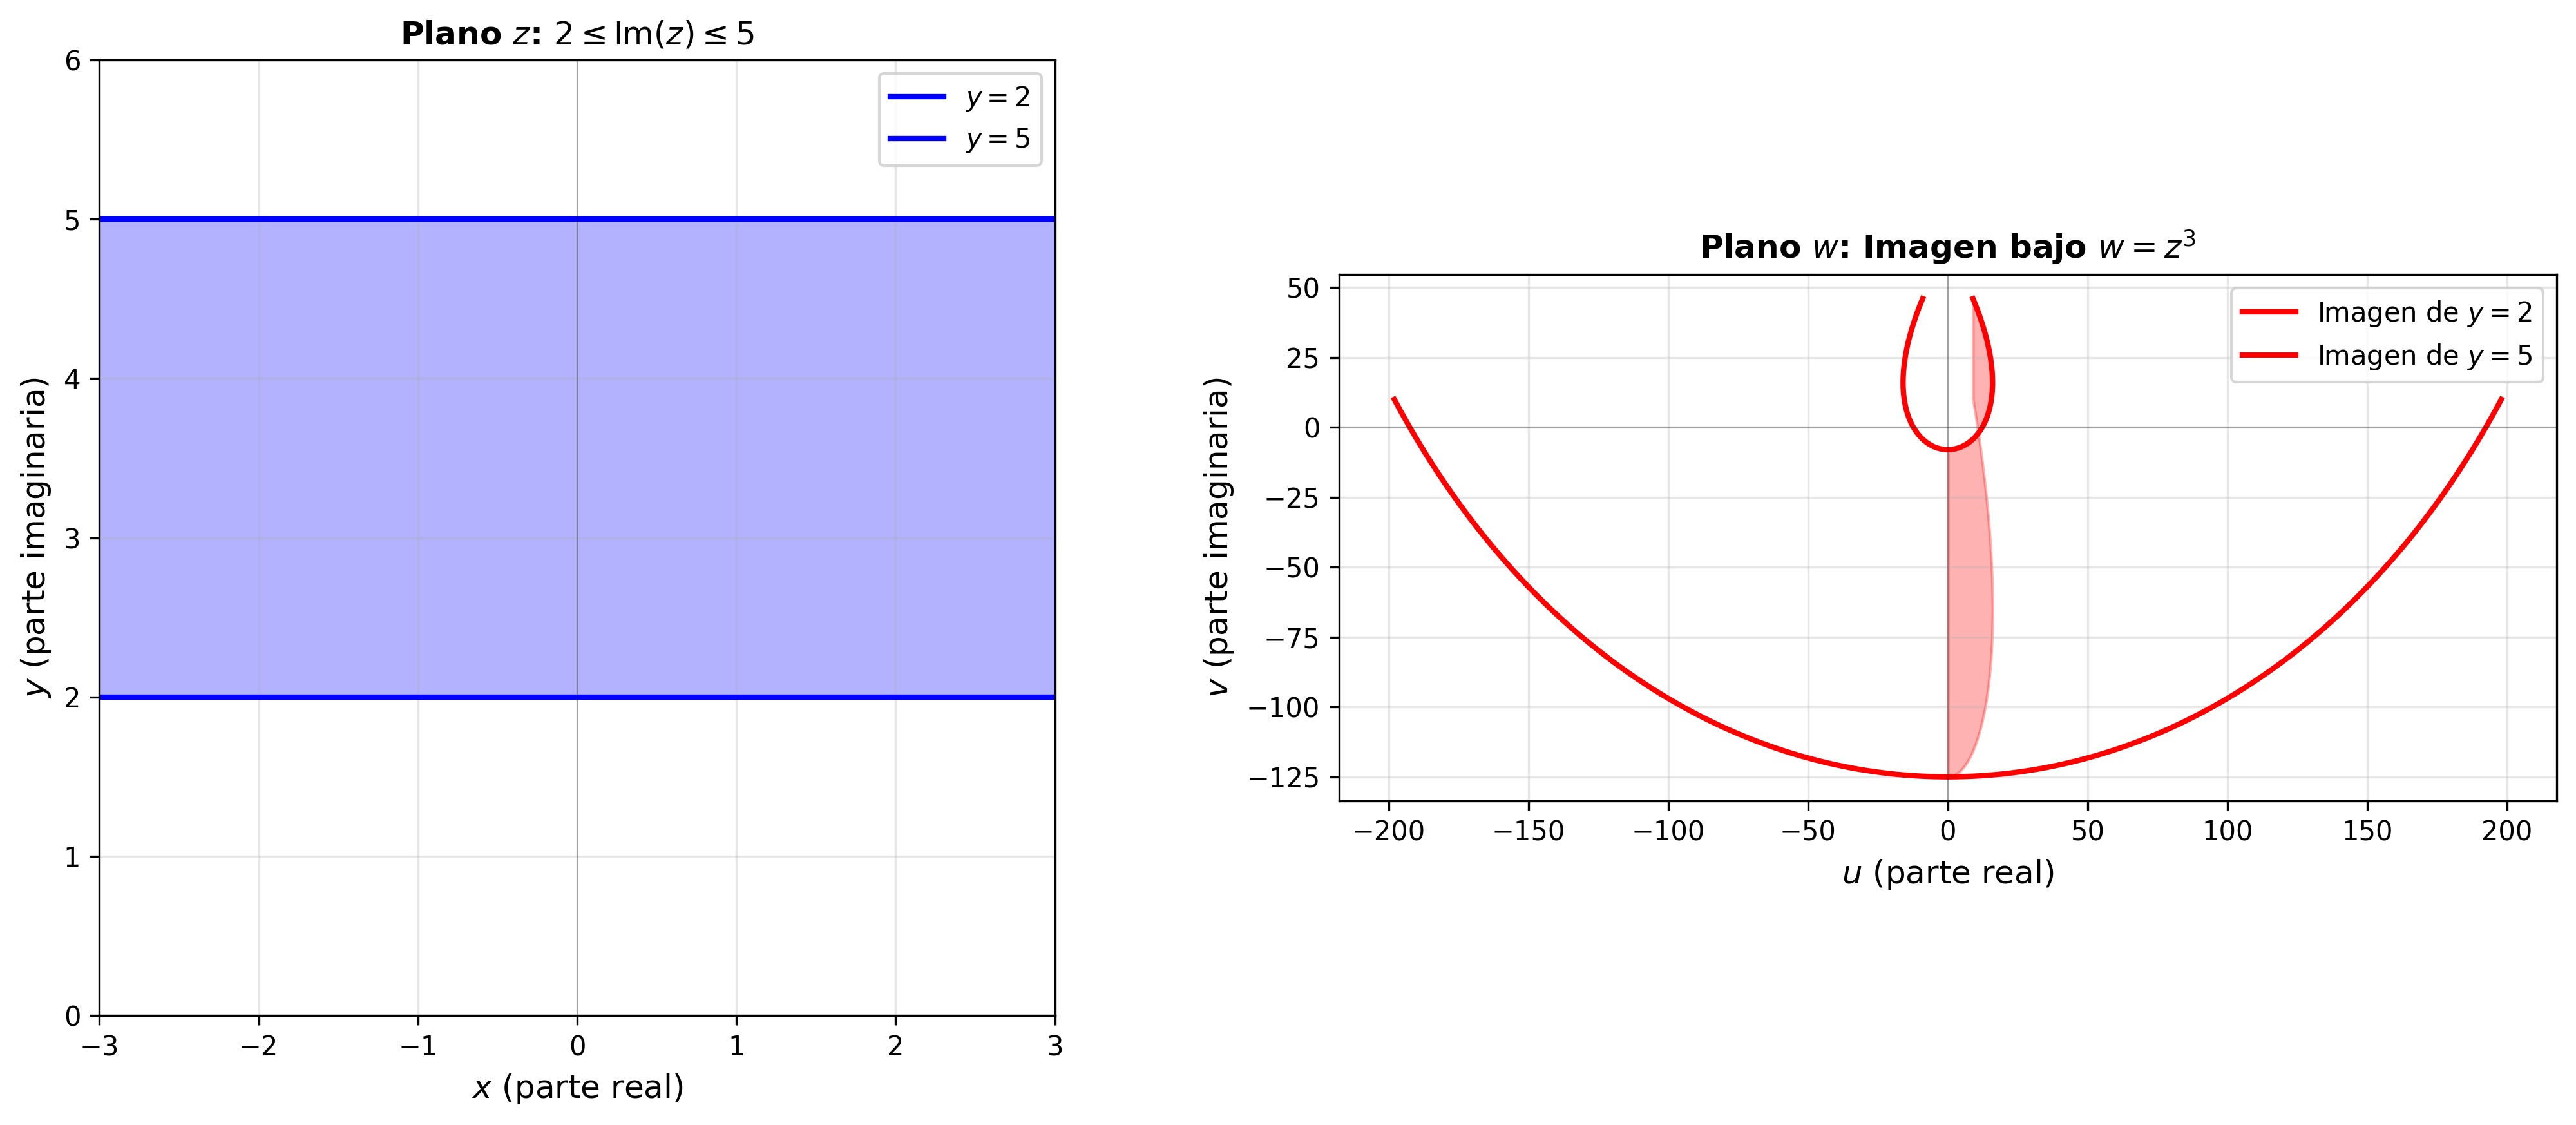
\includegraphics[width=0.9\textwidth]{../Codigos/ejercicio11c.png}
\caption{Región original (izquierda) e imagen transformada (derecha) para el ejercicio 11c.}
\label{fig:ejercicio11c}
\end{figure}

\subsection*{d) Región: $|z - \frac{1}{2}| \leq \frac{1}{2}$; Transformación: $w = \frac{1}{z}$}

\subsubsection*{Descripción de la región en el plano $z$:}

La región está definida por:
\begin{itemize}
\item $|z - \frac{1}{2}| \leq \frac{1}{2}$: disco cerrado de radio $\frac{1}{2}$ centrado en $z = \frac{1}{2}$
\end{itemize}

Este es un \textbf{disco} que toca el origen (ya que el centro está en $\frac{1}{2}$ y el radio es $\frac{1}{2}$, el borde pasa por $z = 0$).

\subsubsection*{Transformación bajo $w = \frac{1}{z}$:}

La transformación $w = \frac{1}{z}$ es una inversión. Para un círculo que pasa por el origen, la imagen es una recta.

Si $z = \frac{1}{2} + re^{i\theta}$ con $r \leq \frac{1}{2}$, entonces el círculo $|z - \frac{1}{2}| = \frac{1}{2}$ pasa por $z = 0$.

Para encontrar la imagen del círculo, usamos la propiedad de que la inversión transforma círculos que pasan por el origen en rectas.

El círculo $|z - \frac{1}{2}| = \frac{1}{2}$ tiene ecuación:
$$(x - \frac{1}{2})^2 + y^2 = \frac{1}{4}$$

Sustituyendo $z = \frac{1}{w} = \frac{1}{u + iv} = \frac{u - iv}{u^2 + v^2}$:
$$x = \frac{u}{u^2 + v^2}, \quad y = -\frac{v}{u^2 + v^2}$$

Sustituyendo en la ecuación del círculo:
$$\left(\frac{u}{u^2 + v^2} - \frac{1}{2}\right)^2 + \left(-\frac{v}{u^2 + v^2}\right)^2 = \frac{1}{4}$$

Simplificando:
$$\frac{u^2 + v^2}{(u^2 + v^2)^2} - \frac{u}{u^2 + v^2} + \frac{1}{4} = \frac{1}{4}$$
$$\frac{1}{u^2 + v^2} - \frac{u}{u^2 + v^2} = 0$$
$$\frac{1 - u}{u^2 + v^2} = 0$$

Por lo tanto, $u = 1$, es decir, $v$ puede ser cualquier valor.

\textbf{Imagen en el plano $w$:} El círculo $|z - \frac{1}{2}| = \frac{1}{2}$ se transforma en la recta $u = 1$ (recta vertical).

El interior del disco se transforma en el semiplano $u \geq 1$ (o $u \leq 1$, dependiendo de la orientación). Para determinar cuál, consideremos un punto interior como $z = \frac{1}{4}$:
$$w = \frac{1}{1/4} = 4$$

Como $u = 4 > 1$, el interior del disco se transforma en el semiplano $u \geq 1$.

\begin{figure}[h]
\centering
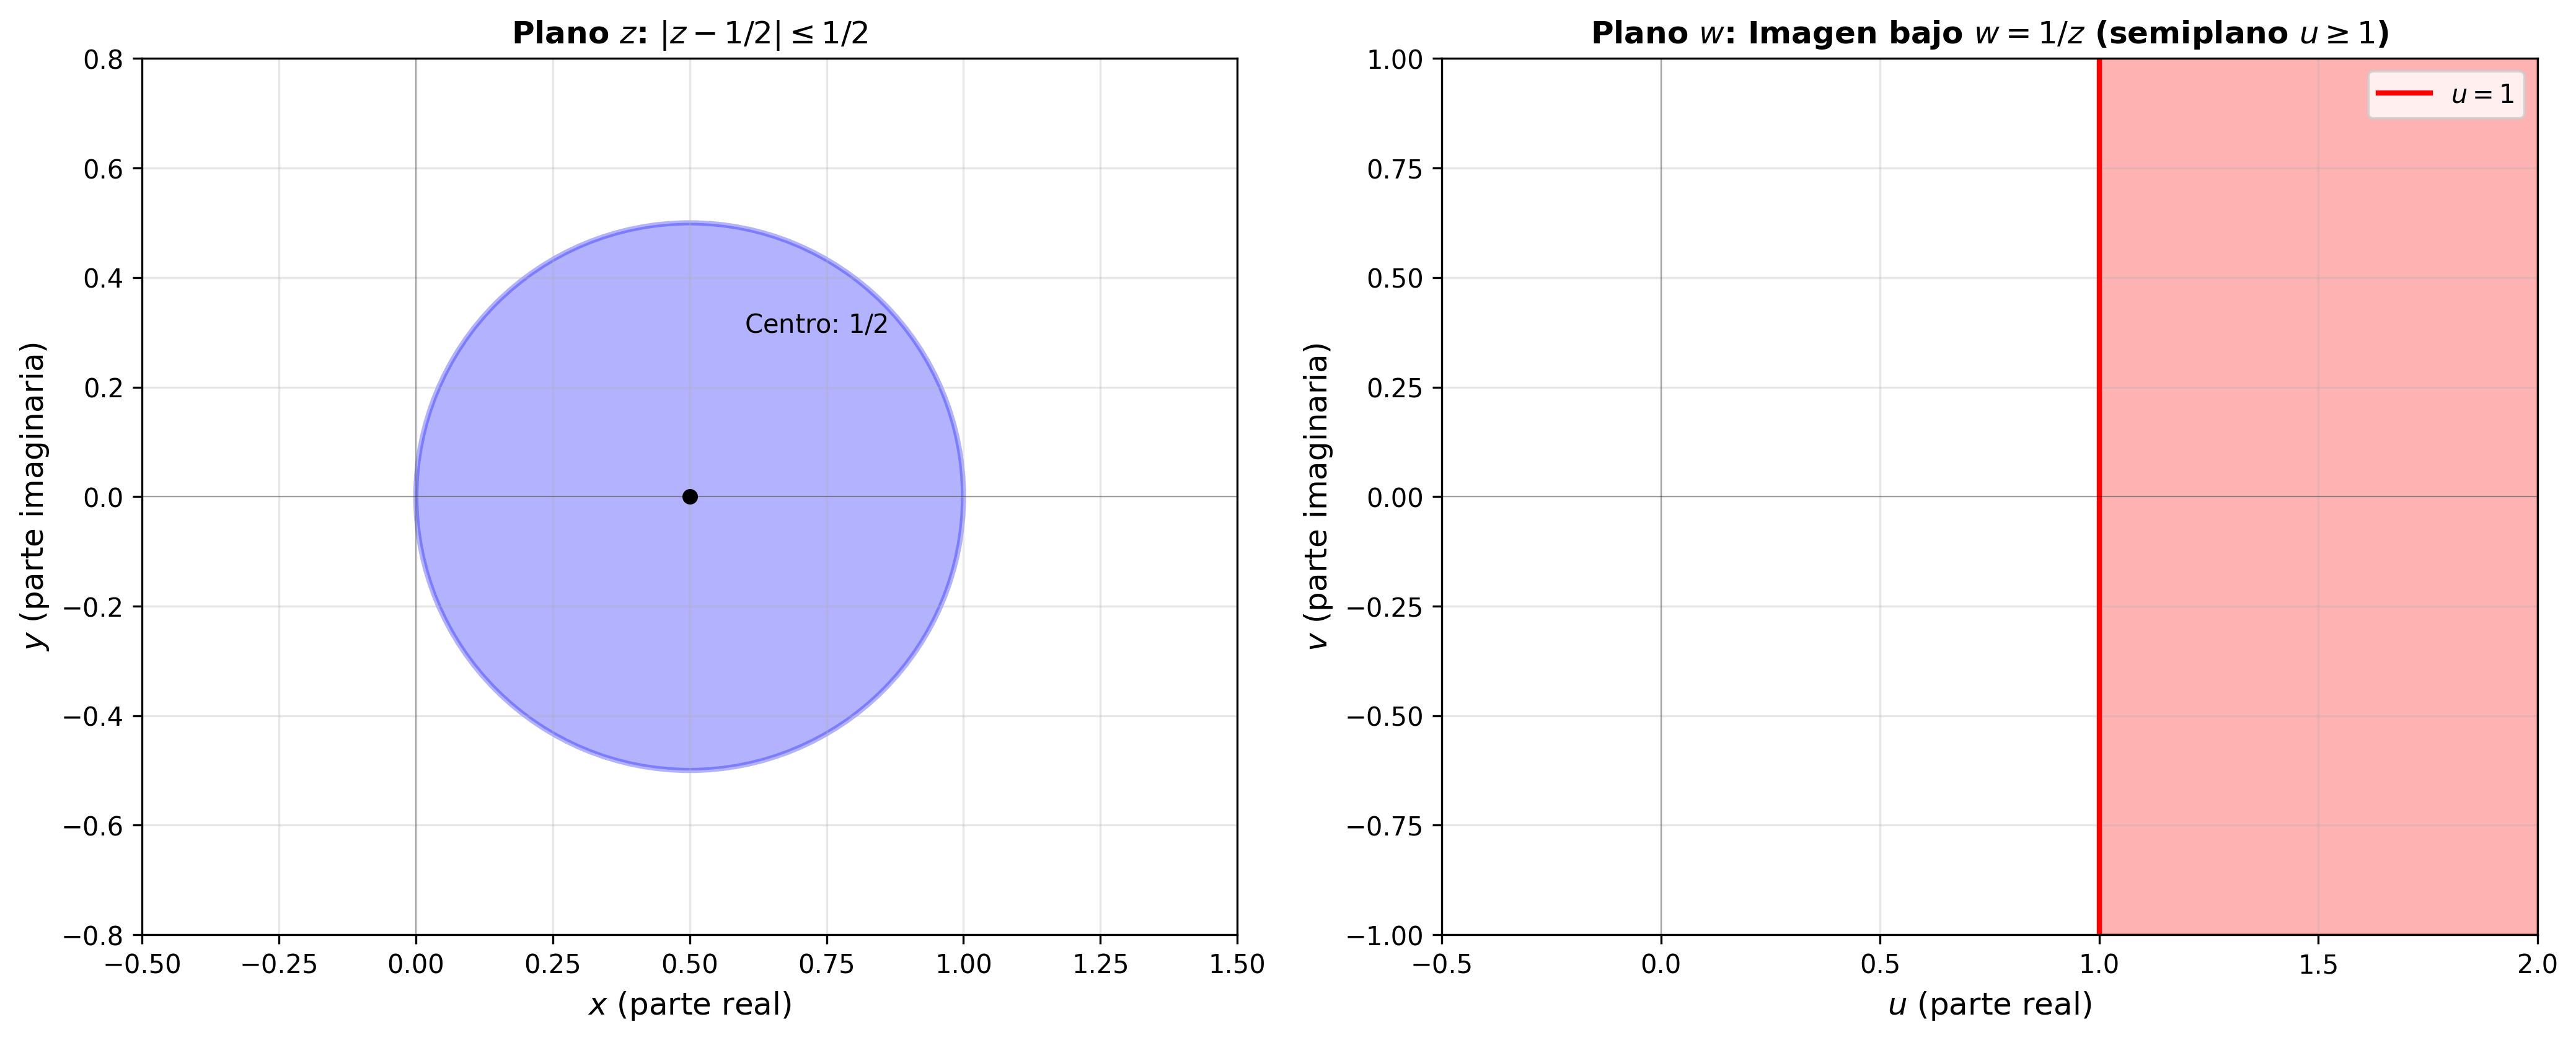
\includegraphics[width=0.9\textwidth]{../Codigos/ejercicio11d.png}
\caption{Región original (izquierda) e imagen transformada (derecha) para el ejercicio 11d.}
\label{fig:ejercicio11d}
\end{figure}

\textbf{Resumen de las transformaciones:}
\begin{itemize}
\item \textbf{(a)} Cuña de radio $\frac{1}{2}$ y ángulo $\frac{\pi}{4}$ $\to$ Cuña de radio $\frac{1}{4}$ y ángulo $\frac{\pi}{2}$
\item \textbf{(b)} Sector de anillo ($1 < r < 3$, $0 < \theta < \frac{\pi}{2}$) $\to$ Sector de anillo ($1 < r < 27$, $0 < \theta < \frac{3\pi}{2}$)
\item \textbf{(c)} Banda horizontal ($2 \leq y \leq 5$) $\to$ Región entre dos curvas cúbicas
\item \textbf{(d)} Disco $|z - \frac{1}{2}| \leq \frac{1}{2}$ $\to$ Semiplanos $u \geq 1$
\end{itemize}

\end{document}

